
%----------------------------------------------------------------------------------------
%   PACKAGES AND OTHER DOCUMENT CONFIGURATIONS
%----------------------------------------------------------------------------------------

\documentclass[paper=a4, fontsize=11pt]{scrartcl} % A4 paper and 11pt font size

\usepackage[T1]{fontenc} % Use 8-bit encoding that has 256 glyphs
\usepackage{fourier} % Use the Adobe Utopia font for the document - comment this line to return to the LaTeX default
\usepackage[english]{babel} % English language/hyphenation
\usepackage{amsmath,amsfonts,amsthm} % Math packages
\usepackage[utf8]{inputenc}
\usepackage{ tipa }
\usepackage{lipsum} % Used for inserting dummy 'Lorem ipsum' text into the template
\usepackage{verbatim}
\usepackage{hyperref}
\usepackage{sectsty} % Allows customizing section commands
\allsectionsfont{\centering \normalfont\scshape} % Make all sections centered, the default font and small caps
\usepackage{graphicx}
\usepackage{fancyhdr} % Custom headers and footers
\pagestyle{fancyplain} % Makes all pages in the document conform to the custom headers and footers
\fancyhead{} % No page header - if you want one, create it in the same way as the footers below
\fancyfoot[L]{} % Empty left footer
\fancyfoot[C]{} % Empty center footer
\fancyfoot[R]{\thepage} % Page numbering for right footer
\renewcommand{\headrulewidth}{0pt} % Remove header underlines
\renewcommand{\footrulewidth}{0pt} % Remove footer underlines
\setlength{\headheight}{13.6pt} % Customize the height of the header
\usepackage{xcolor}
\numberwithin{equation}{section} % Number equations within sections (i.e. 1.1, 1.2, 2.1, 2.2 instead of 1, 2, 3, 4)
\numberwithin{figure}{section} % Number figures within sections (i.e. 1.1, 1.2, 2.1, 2.2 instead of 1, 2, 3, 4)
\numberwithin{table}{section} % Number tables within sections (i.e. 1.1, 1.2, 2.1, 2.2 instead of 1, 2, 3, 4)

\setlength\parindent{0pt} % Removes all indentation from paragraphs - comment this line for an assignment with lots of text
\usepackage{fancyvrb}
\usepackage{anysize}
\marginsize{2cm}{2cm}{1cm}{1cm}
%----------------------------------------------------------------------------------------
%   TITLE SECTION
%----------------------------------------------------------------------------------------

\newcommand{\horrule}[1]{\rule{\linewidth}{#1}} % Create horizontal rule command with 1 argument of height

\title{   
\normalfont \normalsize 
\textsc{Facultad de Ciencias Exactas, Ingeniería y Agrimensura} \\ [25pt] % Your university, school and/or department name(s)
\horrule{0.5pt} \\[0.4cm] % Thin top horizontal rule
\huge Aprendiendo a pronunciar texto en Inglés \\ % The assignment title
\horrule{2pt} \\[0.5cm] % Thick bottom horizontal rule
}

\author{Jeremías Rodríguez} % Your name

\date{\normalsize\today} % Today's date or a custom date

\begin{document}

\maketitle % Print the title

%----------------------------------------------------------------------------------------
%   PROBLEM 1
%----------------------------------------------------------------------------------------

\section{Introducción}

\par La pronunciación del lenguaje inglés ha sido estudiada extensivamente por linguistas, y mucho es sabido sobre las correspondencias entre letras y los sonidos del habla inglesa, llamados \emph{fonemas}.  El inglés es un lenguaje particularmente difícil de dominar por sus irregularidades en la pronunciación. Por ejemplo, la letra "a" en la palabra "gave" es una vocal larga,  pero no en "have" o "read".\\
\par En este trabajo se busca aplicar varios de los contenidos estudiados en este curso (y el anterior) al problema de convertir texto en inglés a su correspondiente transcripción en símbolos fonéticos\footnote{El Alfabeto Fonético Internacional es un sistema de notación fonética creado por lingüistas. Su propósito es otorgar, de forma regularizada, precisa y única, la representación de los sonidos de cualquier lenguaje oral. Tiene aproximadamente 107 símbolos básicos, y cada idioma hace uso de un subconjunto particular.}. \\

\begin{figure}[h!]
\centering
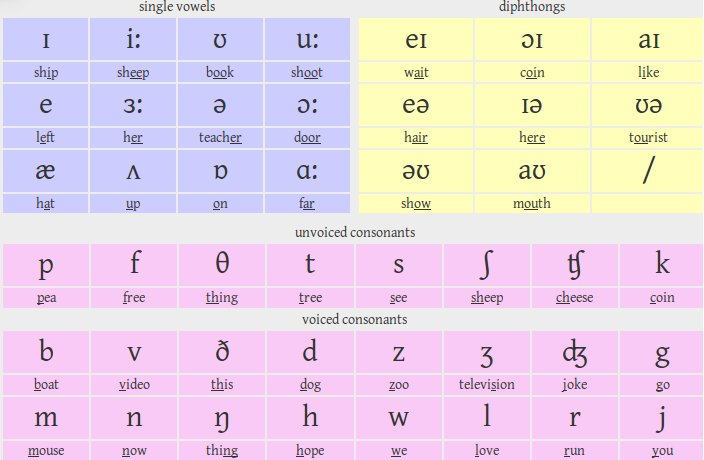
\includegraphics[width=120mm]{phonemicChart.jpg}
\caption{Los 44 sonidos (fonemas) del inglés oral.}
\label{fig:method}
\end{figure}

\par El dataset utilizado se llama netTalk\footnote{\url{https://archive.ics.uci.edu/ml/datasets/Connectionist+Bench+(Nettalk+Corpus)}}, usado por primera vez en el paper  "Parallel Networks that Learn to Pronounce English Text"\cite{parallel}. Los autores lograron entrenar, a partir de unos pocos ejemplos, redes neuronales que convierten strings de texto en inglés (e.g. \textit{calculator}) en strings de fonemas ( $k \ae lkj \omega leIt  \textschwa $) con muchísima precisión.\\
    

\par En este trabajo recrearé y analizaré varios experimentos llevados a cabo en el citado paper; y posteriormente extenderé la investigación utilizando herramientas estudiadas en el curso.

\section{Dataset NetTalk}

\subsection{Presentación del dataset}
El dataset netTalk contiene una fila por cada una de las 20000 palabras del \textit{Miriam Webster’s Pocket Dictionary}. Por cada fila, el dataset contiene sólo dos columnas: \\

\begin{center}

\begin{BVerbatim}
[letter_representation]  [phonemic_representation]
argue                    argY-   
argumentation            argYmxnteS-xn   
argumentative            argYmEntxtIv-   
aright                   xrA--t   
arise                    xrAz-   
aristocracy              @rxstakrxsi   
aristocrat               xrIstxkr@t   
aristocratic             xrIstxkr@tIk   
arithmetic               xrIT-mxtIk   
arithmetical             @rIT-mEtIk-L   
arithmetician            xrIT-mxtIS-xn   
\end{BVerbatim}

\end{center}

Ambas columnas son de tipo string, la primera columna obviamente sólo contiene caracteres del alfabeto inglés (abc..z), mientras que la segunda columna contiene caracteres que representan fonemas. El alfabeto elegido por los autores del paper original cuenta con 50 fonemas, incluyendo algunos fonemas extras utilizados en palabras extranjeras. Los 50 símbolos (fonemas) junto con ejemplos de palabras que utilizan cada uno de estos sonidos puede consultarse en netTalk.names (adjuntado).\\

En el extracto presentado del dataset podemos ver que se ha forzado una correspondencia 1-1 entre letras de una palabra y fonemas de su transcripción: cada fonema de la traducción corresponde a la pronunciación de una de las letras de la palabra inglesa. Por ejemplo, la palabra "arithmetical": 

\begin{center}

\begin{BVerbatim}
a>@ ; r>r ; i>I ; t>T ; h>- ; m>m ; e>E ; t>t; i>I ; c>k ; a>- ; l>l               
\end{BVerbatim}

\end{center}

Esta correspondencia es forzada, por que la cantidad de fonemas usados para pronunciar una palabra podria ser menor a la cantidad de letras de la palabra. Los autores del paper original incluyen un fonema "vacio", representado con el símbolo '-', para indicar la ausencia de sonido. Utilizando este simbolo, se obliga a que la transcripcion fonetica tenga la misma cantidad de caracteres que la palabra original, lo cual es computacionalmente conveniente -como veremos luego-



\subsection{Preprocesamiento}

Todos los métodos que hemos estudiado en Machine Learning y Data Mining requieren que los datos input estén  expresados como una matriz de números reales. El dataset netTalk que se acaba de introducir es una representación a muy alto nivel de la información que queremos utilizar, y por ello los autores del paper original realizaron una codificación y transformación bastante compleja para obtener datos numéricos con los que trabajar. \\

Comencemos por definir claramente lo que queremos obtener. Deseamos hallar una función f que convierta strings con palabras en inglés, a strings con su correspondiente transcripción fonética:

\begin{align*}
  f \colon Words &\to Phonetics \\
  f("hypotenuse") &= "hApat-NYs-".
\end{align*}

Utilizando el hecho de que cada letra del input se corresponde a un fonema en el output, podemos reducir el problema a hallar el fonema correspondiente de una cierta letra de un palabra. Es decir, deseamos obtener una función que se focalice en predecir el fonema de una sóla de las letras a la vez, obviamente teniendo en cuenta el entorno de ella. Asumimos que para predecir el sonido de una letra, sólo necesitamos saber las 3 letras anteriores y las 3 siguientes (si las hay):


\begin{align*}
  g \colon L \times L \times L \times L \times L \times L \times L  & \to Phonems \\
  g(-,-,-,\textcolor{red}{h},y,p,o) &= h \\  
  g(-,-,h,\textcolor{red}{y},p,o,t) &= A \\
  g(-,h,y,\textcolor{red}{p},o,t,e) &= p \\
  g(h,y,p,\textcolor{red}{o},t,e,n) &= a \\
  g(y,p,o,\textcolor{red}{t},e,n,u) &= t \\
  g(p,o,t,\textcolor{red}{e},n,u,s)& = - \\
  g(o,t,e,\textcolor{red}{n},u,s,e)& = N \\
  g(t,e,n,\textcolor{red}{u},s,e,-)& = Y \\
  g(e,n,u,\textcolor{red}{s},e,-,-) &= s
\end{align*}

Por supuesto, esta ventana de 7 letras puede no ser suficiente para algunas palabras donde se necesita considerar una porción más amplia para generar una correcta pronunciación; pero en general funciona bien. Finalmente, si obtenemos esta función g, podemos derivar f aplicando sucesivamente g a cada letra del input de f. 

\begin{align*}
  f("hypotenuse") = g("---\textcolor{red}{h}ypo")  g("--h\textcolor{red}{y}pot") g("-hy\textcolor{red}{p}ote") g("hyp\textcolor{red}{o}ten")  \ldots
\end{align*}


Qué ventajas tiene g respecto a f? Con un input fijo de 7 caracteres y un output fijo de 1 fonema; se puede entrenar un algoritmo de machine learning dándole muchos ejemplos de 7 caracteres y un fonema output correspondiente al caracter central. Aprender la función g es sustancialmente más fácil, porque sólo se predice un caracter a la vez. \\

Por lo tanto, se convirtió el dataset netTalk a un nuevo dataset de 8 columas, donde dividimos cada palabra en varias filas como se ilustró arriba con "hypotenuse". En nuestro caso, de tener 10000 palabras pasamos a tener 146934 filas. Los scripts utilizados en esta fase pueden verse en /src/preprocessing. \\

El paso restante es codificar todos los caracteres de las 146934 filas como números. Para ello usaremos una representación muy simple: Dado que tenemos 26 letras en el alfabeto inglés, reemplazaremos la columna de cada letra por 26 columnas binarias 1-0. Si la primera letra era una 'j', entonces la columna 10 tendrá un 1 y las otras 25 columnas un cero. Los fonemas se codificarán de forma similar, en 20 columnas binarias.\footnote{Los 50 fonemas se codifican en 20 columnas que representan "articulatory features" que los definen, como por ejemplo si tienen un tono alto, medio o bajo; si el ruido procede de la garganta, del paladar, etc; o si el ruido es con o sin voz.} \\

Por lo tanto, nuestro dataset de 146934 filas tendrá 26 * 7 columnas binarias representando las 7 letras input; y otras 20 columnas binarias representando el fonema output. A este dataset resultante le aplicaré las distintas técnicas de aprendizaje y clustering.

\section{Redes Neuronales}
El primer paso es repetir los exprimentos que se realizaron usando redes neuronales en \cite{parallel}. Para ello, utilizaré una red neuronal con 26 * 7 neuronas en la capa de entrada, y 27 en la capa de salida. Repetí los experimentos con distintas cantidades de neuronas en la capa intermedia, para estudiar como cambia la precisión de la red.

\begin{figure}[h!]
\centering
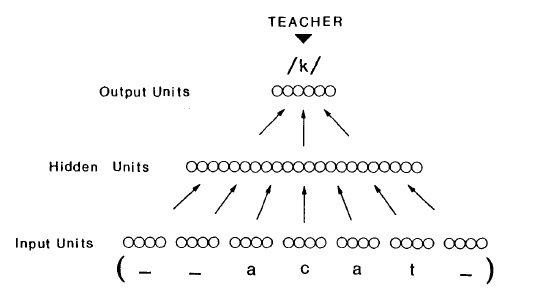
\includegraphics[width=100mm]{figure1.jpg}
\end{figure}


\subsection{Optimización de parámetros}

En un primer experimento dividí aleatoriamente las 20000 palabras originales en 5000 palabras para training/validación y 15000 para testear. Ambos conjuntos fueron preprocesados como se indicó en la sección anterior, para poder entrenar y testear redes neuronales. \\

Los dos parámetros a optimizar, learning rate y momentum, fueron elegidos utilizando grid search. Realicé la búsqueda para $\mu$ y $\eta$ entre  $10^0 y 10^{-7}$ (49 combinaciones), y dado que entrenar cada red tarda un tiempo muy considerable y se deben realizar varias corridas, decidí utilizar sólo 20 neuronas en la capa intermedia para esta etapa de optimización de parámetros. \\

Utilicé el algoritmo backpropagation, en particular la implementación en C que utilizamos en el curso de machine learning. Dividí el conjunto de 5000 palabras en 4000 para training y 1000 para validación. Una vez obtenida la salida de la red (.predict), discreticé el resultado y calculé el error discreto en test. Toda esta etapa precisó más de 50hs de cpu utilizando una procesador intel i7 con 8 cores. Los parámetros óptimos fueron e=0.1 y u=0.000001 y el código de toda esta sección puede verse en /src/ANNs

\subsection{Complejidad de la red neuronal}
Una vez seleccionados los parámetros óptimos, el siguiente paso fue entrenar redes de tamaño mucho más grande  y con muchas más épocas. Para cada configuración de red, se entrenaron varias redes y se eligió aquella que presentó el máximo error en test.  La siguiente tabla resume los resultados:

\begin{center}
\begin{tabular}{ |c| c|  }
\hline
Neuronas en la capa intermedia & \% accuracy in test \\
\hline 
20  & 0.7525778  \\
50  & 0.8457043  \\
100 & 0.8548013  \\
150 & 0.8457043  \\
\hline
\end{tabular}
\end{center}


Como vemos, usando una red con más de 50 neuronas podemos llegar a un accuracy realmente alto. Sin embargo, se aprecia que seguir agregando más neuronas no contribuye seguir mejorando el resultado. \\

Me parece asombroso llegar a predecir con tanta exactitud los fonemas, dado que este problema es muy complejo y posee una gran cantidad de reglas y excepciones. Para aumentar aún más el valor de accuracy, puede ser interesante aplicar a la red la mejora de weight decay que estudiamos en machine learning, realizar un ajuste de parámetros más fino o ampliar la cantidad de neuronas de entrada (en vez de utilizar una ventana de 7 dígitos, utilizar más). En el paper original se alcanzan porcentajes similares, e incluso se llega superar el 90\% entrenando la red con más de 30000 épocas.\\

\subsection{Tamaño del conjunto de entrenamiento}
Un último experimento que me resultó interesante de realizar con redes neuronales es probar cuánto se puede aprender de la pronunciación del lenguaje inglés si utilizamos conjuntos más y más pequeños para entrenar. Los experimentos se realizaron con redes de 100 neuronas ocultas:


\begin{center}
\begin{tabular}{ |c|c|c|  }
\hline
Cardinal conjunto training & Número de palabras en training & \% accuracy in test \\
\hline 
30000 & 4500 & 0.8548013  \\
5000  & 750  & 0.7921189 \\
1000  & 150  & 0.6648153  \\
\hline
\end{tabular}
\end{center}

En la primera fila, el conjunto de training de 4500 palabras es codificado en 30000 filas, y la red neuronal de 100 neuronas ocultas realiza una predicción muy buena. \\

Sin embargo, me resulta mucho más asombroso que las otras dos filas den resultados tan buenos. Con sólo 750 palabras del idioma somos capaces de predecir la pronunciación del resto del idioma con casi 80\% de precisión. Incluso con una pequeña muestra de la pronunciación inglesa (150 palabras) el resultado sigue siendo razonable.\\


\subsection{Ejemplos y conclusión}

Esta tarea exhibe una gran cantidad de regularidades globales junto con reglas más especializadas y casos excepcionales. Los resultados fueron muy buenos y las redes aprendieron exitosamente a generar una pronunciación cercana a la real. Veamos algunos ejemplos:

\begin{center}
\begin{BVerbatim}
Written Representation  predicted Phonetics   real Phonetics  
machine                 m@C-en-               mxS-in-  
learning                lI-rnIG-              l--RnIG- 
unexpected              xnEXpEktxd            xnIXpEktxd  
beautiful               bcc-tIfcl             bY--tIf^l 
telescope               tIlEskxp-             tElxskop- 
virus                   varxs                 vArxs

\end{BVerbatim}
\end{center}


Como se puede apreciar, la red se confunde en varios fonemas, pero los errores son muy similares a los que cometemos las personas, pues la confusión se da generalmente entre vocales con sonidos similares. \\

Me interesaría mucho saber si este mismo procedimiento funcionaría para aprender cualquier idioma, provisto un dataset de palabras y sus transcripciones fonéticas.

\section{Random Forest}

Utilizando el dataset codificado, con 5000 palabras codificadas en el conjunto de training, decidí aplicar el algoritmo random forest.\\
Dado que hay 20 columnas binarias de output, entrené 20 clasificadores, cada uno especializado en predecir la columna i-ésima. \\
Finalmente, combiné los resultados de los 20 clasificadores para generar las predicciones completas del conjunto de 15000 palabras test. El tiempo de entrenamiento fue similar al de redes neuronales, pues hubo que entrenar 20 clasificadores. Utilicé 500 árboles por ensemble.\\








\begin{thebibliography}{9}
\bibitem{parallel} 
Terrence J. Sejnowski and Charles R. Rosenberg
\textit{Parallel Networks that Learn to Pronounce English Text}. 
Complex Systems 1 (1987)
 

\end{thebibliography}

\end{document}
